\documentclass[aspectratio=169,11pt]{beamer}

% ── Theme & Colors ──────────────────────────────────────────────
\usetheme{Madrid}
\usecolortheme{whale}

\definecolor{darkblue}{RGB}{0,51,102}
\definecolor{accentblue}{RGB}{51,122,183}
\definecolor{lightgray}{RGB}{245,245,245}
\definecolor{alertred}{RGB}{192,57,43}
\definecolor{successgreen}{RGB}{39,174,96}

\setbeamercolor{palette primary}{bg=darkblue, fg=white}
\setbeamercolor{palette secondary}{bg=accentblue, fg=white}
\setbeamercolor{frametitle}{bg=darkblue, fg=white}
\setbeamercolor{title}{bg=darkblue, fg=white}
\setbeamercolor{block title}{bg=accentblue, fg=white}
\setbeamercolor{block body}{bg=lightgray, fg=black}
\setbeamercolor{block title alerted}{bg=alertred, fg=white}
\setbeamercolor{block body alerted}{bg=lightgray, fg=black}
\setbeamercolor{block title example}{bg=successgreen, fg=white}
\setbeamercolor{block body example}{bg=lightgray, fg=black}
\setbeamercolor{item}{fg=accentblue}

\setbeamertemplate{navigation symbols}{}
\setbeamertemplate{footline}{%
  \leavevmode\hbox{%
    \begin{beamercolorbox}[wd=.33\paperwidth,ht=2.5ex,dp=1ex,center]{palette primary}%
      \usebeamerfont{author in head/foot}\insertshortauthor
    \end{beamercolorbox}%
    \begin{beamercolorbox}[wd=.34\paperwidth,ht=2.5ex,dp=1ex,center]{palette secondary}%
      \usebeamerfont{title in head/foot}\insertshorttitle
    \end{beamercolorbox}%
    \begin{beamercolorbox}[wd=.33\paperwidth,ht=2.5ex,dp=1ex,right]{palette primary}%
      \insertframenumber{} / \inserttotalframenumber\hspace*{2ex}
    \end{beamercolorbox}}%
}

% ── Packages ────────────────────────────────────────────────────
\usepackage[T1]{fontenc}
\usepackage[utf8]{inputenc}
\usepackage{booktabs}
\usepackage{tikz}
\usetikzlibrary{arrows.meta,positioning,shapes.geometric,calc}
\usepackage{mathtools}

% ── Meta ────────────────────────────────────────────────────────
\title[PR Communication Tone]{Communication Tone, Pull Request Outcomes,\\and Contributor Return in Open Source Software
\newline
Part 2: Mid-term Presentation}
\author[D.S Bouras]{Dimitrios Stamatios Bouras}
\institute{Quantitative Analysis of Open Source Software
\newline
Student Number: 2501112125}
\date{2026 / 05 / 6}

% ════════════════════════════════════════════════════════════════
\begin{document}

% ── Title ───────────────────────────────────────────────────────
\begin{frame}
\titlepage
\end{frame}

% ════════════════════════════════════════════════════════════════
% PART 1
% ════════════════════════════════════════════════════════════════
\begin{frame}
\vfill
\begin{center}
  {\Large\bfseries\color{accentblue} Part 1}\\[0.5em]
  {\large What question are we tackling?}\\[0.3em]
  {\color{darkblue}\rule{0.55\textwidth}{0.6pt}}
\end{center}
\vfill
\end{frame}

% ── Part 1: Research Question ────────────────────────────────────
\begin{frame}{Part 1\\Research Question and Background}

\begin{block}{Central question}
Are communication signals in PR discussion associated with
\textbf{merge outcomes} and \textbf{contributor return}?
\end{block}

\vspace{0.2em}
\textbf{Four research questions}
\begin{description}
  \item[RQ1] Which signals are associated with \textbf{PR merge}?
  \item[RQ2] Which signals are associated with \textbf{author return} (30 / 90 / 180 days)?
  \item[RQ3] Do \textbf{newcomers} experience or respond to discussion differently?
  \item[RQ4] Does \textbf{politeness} moderate the association between harsh language and return?
\end{description}

\vspace{0.2em}
\begin{alertblock}{Study framing}
Observational: \emph{which discussion signals associate with outcomes?}
\end{alertblock}

\end{frame}

% ════════════════════════════════════════════════════════════════
% PART 2
% ════════════════════════════════════════════════════════════════
\begin{frame}
\vfill
\begin{center}
  {\Large\bfseries\color{accentblue} Part 2}\\[0.5em]
  {\large What research progress has been made?}\\[0.3em]
  {\color{darkblue}\rule{0.55\textwidth}{0.6pt}}
\end{center}
\vfill
\end{frame}

% ── Part 2: Pipeline and Data ────────────────────────────────────
\begin{frame}{Part 2\\Pipeline Built — Data Collected}

{\centering
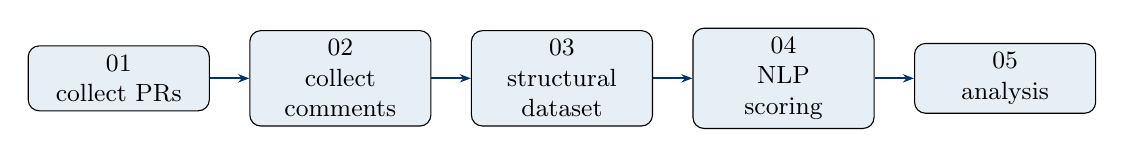
\begin{tikzpicture}[
  box/.style={draw, rounded corners, fill=accentblue!12, minimum width=2.3cm,
              minimum height=0.75cm, align=center, font=\small},
  arr/.style={-{Stealth[length=4pt]}, thick, darkblue}
]
\node[box] (a) {01\\collect PRs};
\node[box, right=0.5cm of a] (b) {02\\collect\\comments};
\node[box, right=0.5cm of b] (c) {03\\structural\\dataset};
\node[box, right=0.5cm of c] (d) {04\\NLP\\scoring};
\node[box, right=0.5cm of d] (e) {05\\analysis};
\draw[arr] (a) -- (b); \draw[arr] (b) -- (c);
\draw[arr] (c) -- (d); \draw[arr] (d) -- (e);
\end{tikzpicture}\par}

\vspace{-0.3em}
\begin{columns}[T]
\begin{column}{0.48\textwidth}
\begin{exampleblock}{Dataset scale}
\begin{itemize}
  \item \textbf{12,098} focal PRs (Jan 2024 -- Mar 2025)
  \item \textbf{3} repositories: Kubernetes, Next.js, scikit-learn
  \item \textbf{2,210} distinct PR authors
  \item \textbf{100k+} comments scored with NLP
\end{itemize}
\end{exampleblock}
\end{column}

\begin{column}{0.48\textwidth}
\begin{block}{Signals computed per PR}
\begin{itemize}
  \item toxicity (mean, max, binary flags)
  \item sentiment
  \item anger
  \item politeness
\end{itemize}
\end{block}
\begin{exampleblock}{Status}
Full pipeline complete; preliminary analysis running.
\end{exampleblock}
\end{column}
\end{columns}

\end{frame}

% ── Part 2: Early Signals ────────────────────────────────────────
\begin{frame}{Part 2\\What the Data Looks Like So Far}

\begin{columns}[T]
\begin{column}{0.52\textwidth}
\textbf{Descriptive picture}
\begin{itemize}
  \item Merge rate: $\sim$\textbf{76\%} across repositories
  \item Return rates are high — majority of authors return within 90 days
  \item Overt toxicity is \textbf{very sparse}: $<$1\% of PRs exceed common thresholds
  \item Sentiment slightly negative; anger and politeness vary more widely
\end{itemize}

\begin{alertblock}{Early pattern}
Preliminary models: \textbf{contributor experience} dominates return.
Communication signals carry more signal for \textbf{merge} than for return.
\end{alertblock}
\end{column}

\begin{column}{0.44\textwidth}
\begin{block}{Outcome rates (preliminary)}
\begin{center}
\small
\begin{tabular}{lr}
\toprule
\textbf{Outcome} & \textbf{Rate} \\
\midrule
Merge         & 75.7\% \\
Return 30d    & 76.8\% \\
Return 90d    & 81.3\% \\
Return 180d   & 83.5\% \\
\midrule
Toxic $\geq$0.05 & 1.0\% \\
\bottomrule
\end{tabular}
\end{center}
\end{block}
\end{column}
\end{columns}

\end{frame}

% ════════════════════════════════════════════════════════════════
% PART 3
% ════════════════════════════════════════════════════════════════
\begin{frame}
\vfill
\begin{center}
  {\Large\bfseries\color{accentblue} Part 3}\\[0.5em]
  {\large Challenges encountered and adjustments made}\\[0.3em]
  {\color{darkblue}\rule{0.55\textwidth}{0.6pt}}
\end{center}
\vfill
\end{frame}

% ── Part 3: Toxicity challenge ───────────────────────────────────
\begin{frame}{Part 3\\Operationalizing Toxicity: From Average to Maximum}

\begin{columns}[T]
\begin{column}{0.50\textwidth}
\begin{alertblock}{What the data revealed}
Mean toxicity per PR is near zero almost everywhere.
Averaging washes out rare but impactful hostile comments.
\end{alertblock}

\begin{exampleblock}{Design choice}
Primary emphasis placed on:
\begin{itemize}
  \item \textbf{max toxicity} per PR — captures worst-case exposure
  \item \textbf{binary indicators}: any comment $\geq 0.05$, any $\geq 0.10$
  \item both used as robustness checks against each other
\end{itemize}
\end{exampleblock}
\end{column}

\begin{column}{0.46\textwidth}
\begin{block}{Why max toxicity}
A single hostile comment can affect a contributor's experience.
The average never reveals it; the maximum does.
\end{block}

\vspace{0.3em}
\begin{block}{Broader signal picture}
Sentiment, anger, and politeness vary more widely than toxicity
and carry more usable signal across all RQs.
\end{block}
\end{column}
\end{columns}

\end{frame}

% ── Part 3: Newcomer + controls ──────────────────────────────────
\begin{frame}{Part 3\\Classifying Experience and Controlling for Confounds}

\begin{columns}[T]
\begin{column}{0.50\textwidth}
\begin{alertblock}{Newcomer definition requires care}
A first-PR rule mislabels contributors who were active before the collection window.
\end{alertblock}

\vspace{0.2em}
\begin{exampleblock}{6-month lookback window}
Collection extended to \textbf{Jul 2023}; focal PRs start \textbf{Jan 2024}.\\
The Jul--Dec 2023 buffer provides prior history to classify contributors reliably.\\
Same design ensures \textbf{complete 180-day return labels} for all focal PRs.
\end{exampleblock}
\end{column}

\begin{column}{0.46\textwidth}
\begin{block}{Known limitation: NLP domain}
Pre-trained models were trained on social media. In code review, \emph{``this is completely broken''} is
technical criticism, not hostility. Scores are used directly; this is acknowledged as a limitation.
\end{block}

\vspace{0.2em}
\begin{block}{Added controls}
Contributor history, discussion size, first-response delay, and repository fixed effects
included to isolate the communication signal.
\end{block}
\end{column}
\end{columns}

\end{frame}

% ════════════════════════════════════════════════════════════════
% PART 4
% ════════════════════════════════════════════════════════════════
\begin{frame}
\vfill
\begin{center}
  {\Large\bfseries\color{accentblue} Part 4}\\[0.5em]
  {\large Future research plans}\\[0.3em]
  {\color{darkblue}\rule{0.55\textwidth}{0.6pt}}
\end{center}
\vfill
\end{frame}

% ── Part 4: Future Plans ─────────────────────────────────────────
\begin{frame}{Part 4\\What Comes Next}

\begin{columns}[T]
\begin{column}{0.50\textwidth}
\textbf{Analysis to complete}
\begin{itemize}
  \item Finalize logistic regressions for all 4 RQs with full controls
  \item Run binary toxicity robustness checks
  \item Test newcomer $\times$ toxicity interaction (RQ3)
  \item Confirm politeness moderation result (RQ4)
\end{itemize}
\end{column}

\begin{column}{0.46\textwidth}
\textbf{Interpretation and write-up}
\begin{itemize}
  \item Present findings clearly for each RQ
  \item Keep only figures that communicate a clear result
  \item Discuss limitations:
  \begin{itemize}
    \item PR-only return definition
    \item Sparse toxicity limits power
    \item NLP–domain mismatch
    \item Observational design only
  \end{itemize}
\end{itemize}
\end{column}
\end{columns}

\vspace{0.2em}
\begin{exampleblock}{Expected findings}
Communication signals associate more strongly with \textbf{merge outcome} than with contributor return.
Contributor experience and history are the dominant predictors of return.
\end{exampleblock}

\end{frame}

% ── Closing ─────────────────────────────────────────────────────
\begin{frame}
\vfill
\begin{center}
  {\Huge\bfseries Thank you}\\[0.8em]
  {\large Questions?}
\end{center}
\vfill
\end{frame}

\end{document}
